\chapter{An Example}
This section will present a pedagogically interesting 
example which demonstrates several of the program's important
features.  The purpose of this chapter is neither to be 
comprehensive nor to be particularly detailed. It will instead 
give a sense of the types of analysis that can be done with 
this program. It will act as a motivation for the rest of the manual. 
Further details 
and information on any of the things described below can be found in 
the appropriate sections of the manual.

David, a user of the program, was studying iron thin films 
using powder diffraction. He was particularly interested in 
measuring the shift in diffraction peaks of his sample. To 
realize this experimentally, he capture data of the 
calibration standard Lanthanum Hexaboride (LaB6). 
Without changing the experimental parameters, he then imaged 
many samples that he wanted to analyze. 

\begin{SCfigure}[1][bthp]
    \centering
    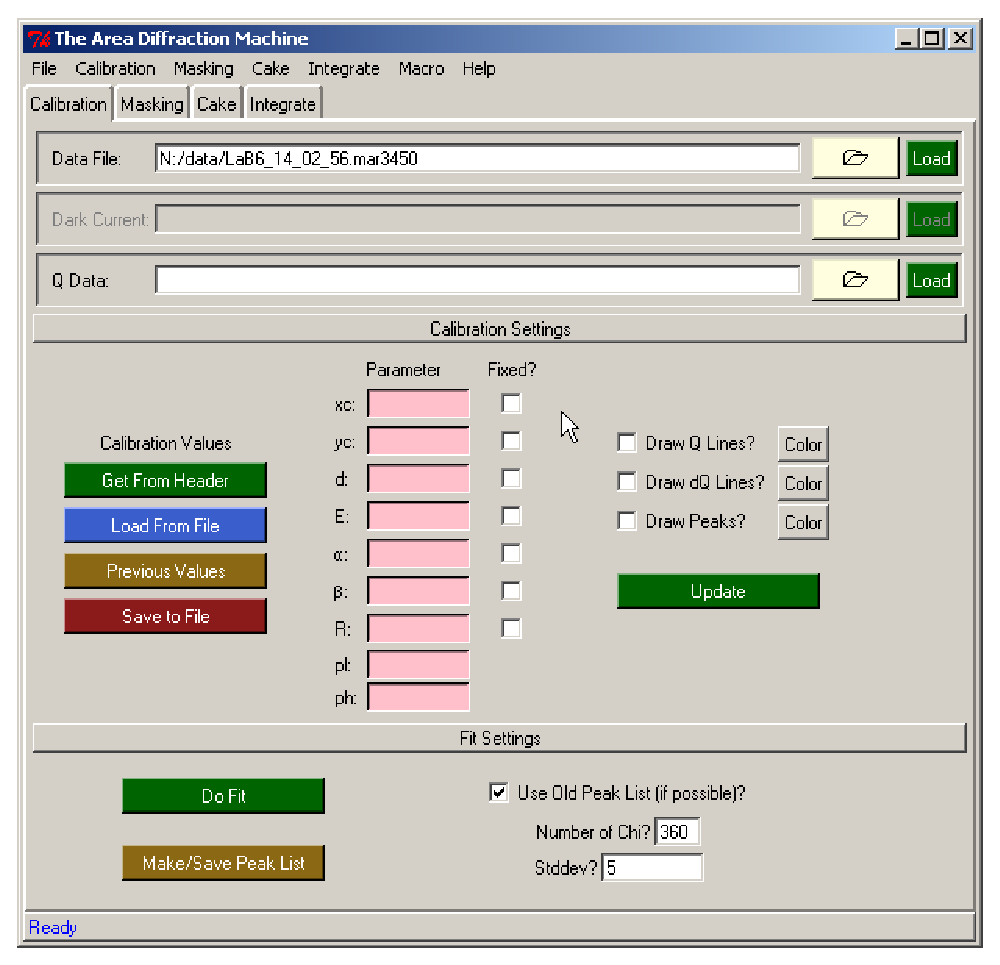
\includegraphics[scale=.75]
    {figures/calibration_tab.eps}
    \caption{The calibration tab.}
    \label{calibration_tab_example}
\end{SCfigure}

\begin{SCfigure}[1][bthp]
    \centering
    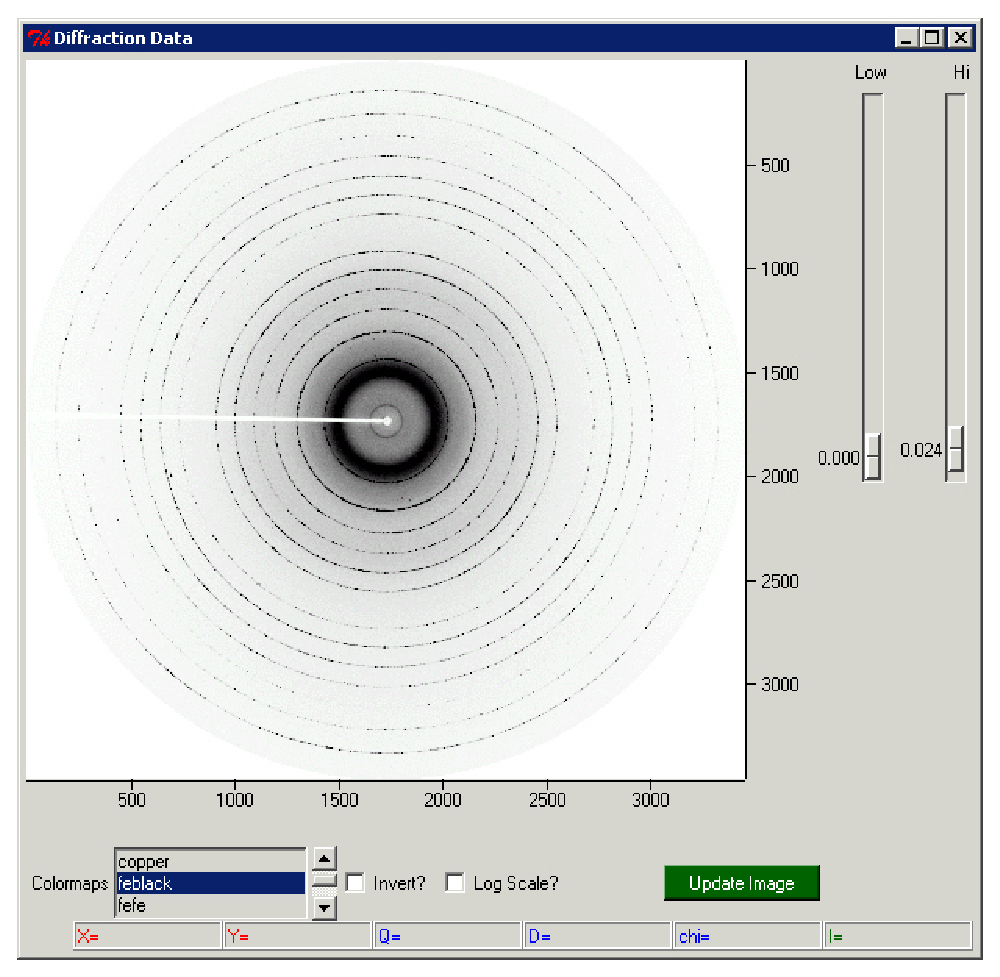
\includegraphics[scale=.75]
    {figures/diffraction_data_window_example.eps}
    \caption{The diffraction data window.}
    \label{diffraction_data_window_example}
\end{SCfigure}

The steps needed to do this analysis will be
described. First, The diffraction detector needs to be calibrated.
This will determine the precise experimental parameters that 
characterize the diffraction machine when the data was captured.
Since the image of the standard was taken at the same
time as the other images, the calibration parameters inferred
from the standard crystal can be used to analyze the rest of data.
Figure~\ref{calibration_tab_example} shows what 
is first displayed when the Area Diffraction Machine is first
opened. Using the \gui{Data File} input, the LaB6
file can be loaded. 
Figure~\ref{diffraction_data_window_example} shows a new
window that opens up with the diffraction data.
To calibrate the detector, the program must know the 
$Q$ values for the standard crystal. Since LaB6 is so common, it is
a preset default in the program. Figure~\ref{standard_q_example}
shows how to do this.

\begin{SCfigure}[1][bthp]
    \centering
    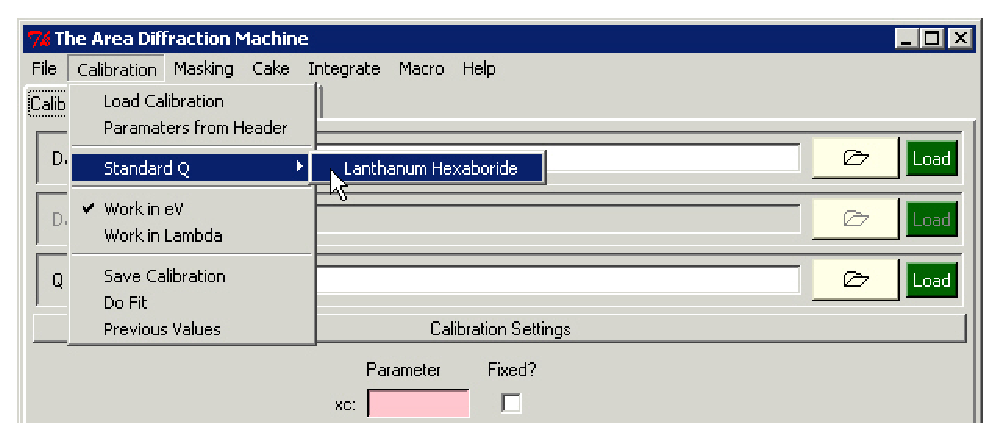
\includegraphics[scale=.75]
    {figures/standard_q.eps}
    \caption{Loading a standard $Q$ file.
    (More standard $Q$ files might be added in the future).}
    \label{standard_q_example}
\end{SCfigure}

The program also
needs an initial guess of the calibration parameters. 
Decent guesses at the experimental parameters are often
stored in the diffraction data's header. 
The program can try to find these values with the 
\gui{Get From Header} button. After the image, the $Q$ values, 
and an initial guess at the parameters have been loaded, 
the detector can be calibrated.

But first, the quality of the initial guess can be checked
with the \gui{Draw Q Lines?}
check box on the \gui{Calibration} tab. The program will draw
on top of the diffraction image what pattern should show 
up on the detector (for the given calibration parameters and $Q$
values). Figure~\ref{bad_calibration_diffraction_image}
shows an example. Of course, the initial guess isn't
great. 

\begin{SCfigure}[1][bthp]
    \centering
    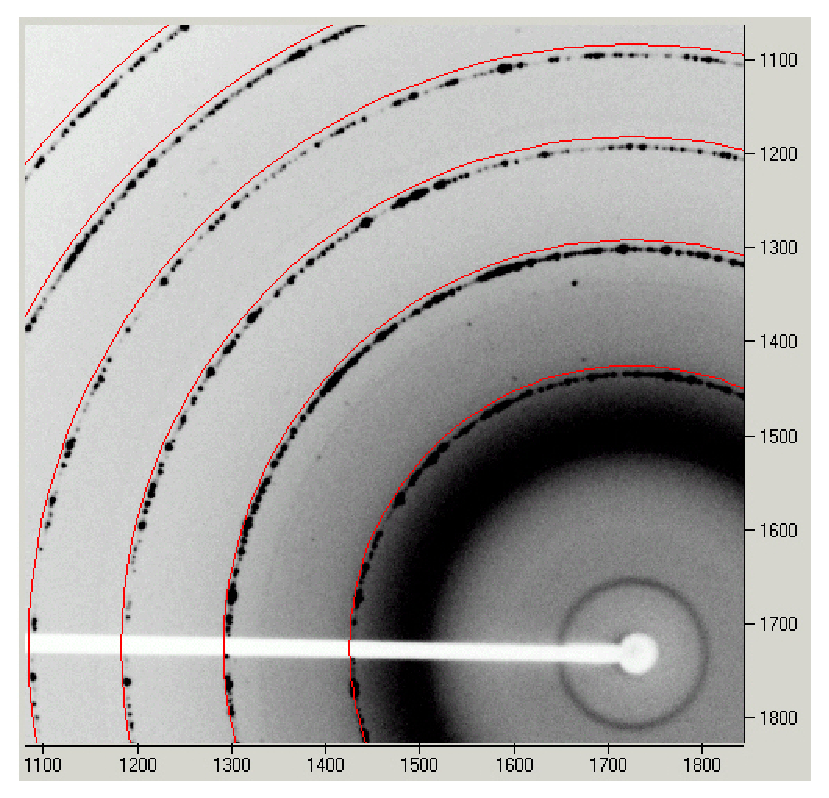
\includegraphics[scale=.75]
    {figures/bad_calibration_diffraction_image.eps}
    \caption{The diffraction image with constant $Q$
    lines displayed on it. These lines were calculated
    for the calibration parameters found in the
    image header and are not particularly accurate.}
    \label{bad_calibration_diffraction_image}
\end{SCfigure}

The diffraction data can be caked. 
If the calibration parameters are known exactly, 
the diffraction peaks will show up as many vertical lines.
If the parameters are not exact, the diffraction peaks
will have a distortion to them.
The data can be caked on the \gui{Cake} tab using the 
\gui{AutoCake} button and a new window will open. 
this tab is shown in figure~\ref{cake_tab_example} 
and the cake window is shown in 
figure~\ref{bad_calibration_cake}.
The diffraction peaks on the caked data with the header 
calibration parameters are not very straight. They have a
systematic wiggle. 
Figure~\ref{bad_calibration_cake_zoom} shows that this 
this distortion becomes very obvious when one peak is
zooomed into.


\begin{SCfigure}[1][bthp]
    \centering
    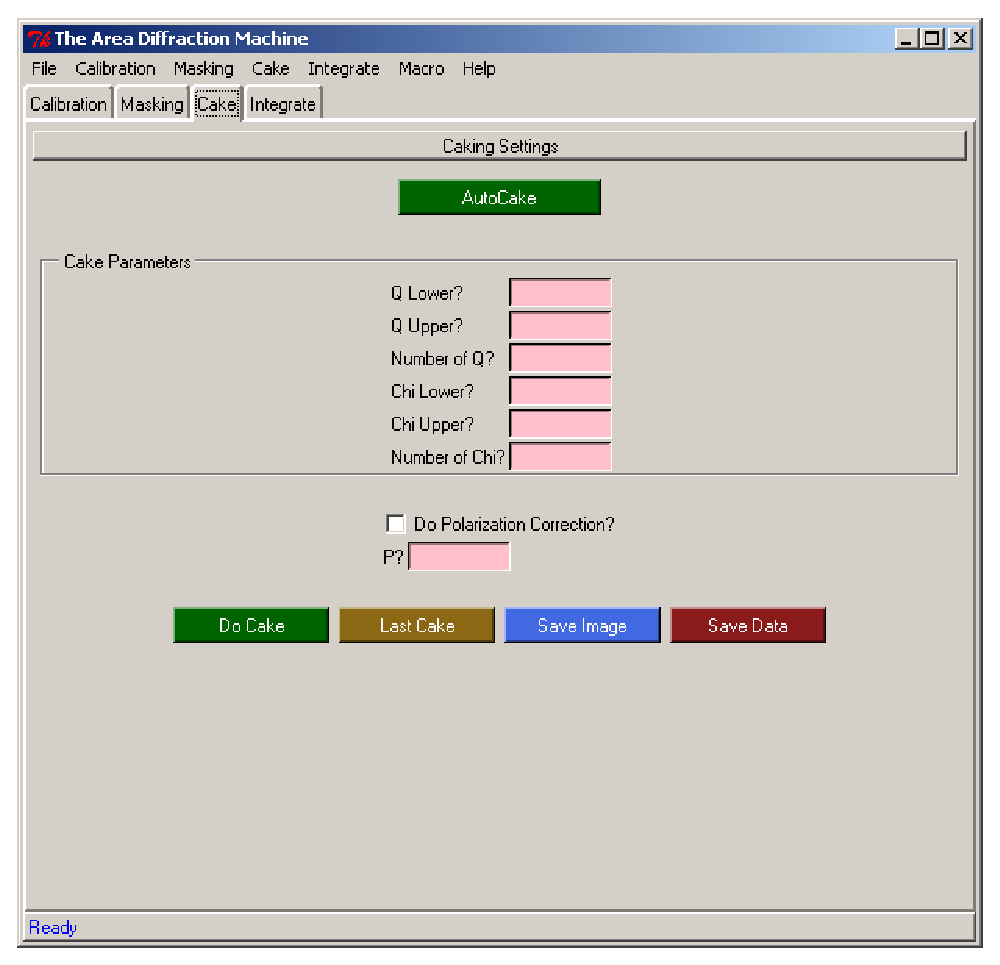
\includegraphics[scale=.75]
    {figures/caking_tab.eps}
    \caption{The calibration tab.}
    \label{cake_tab_example}
\end{SCfigure}

\begin{SCfigure}[1][bthp]
    \centering
    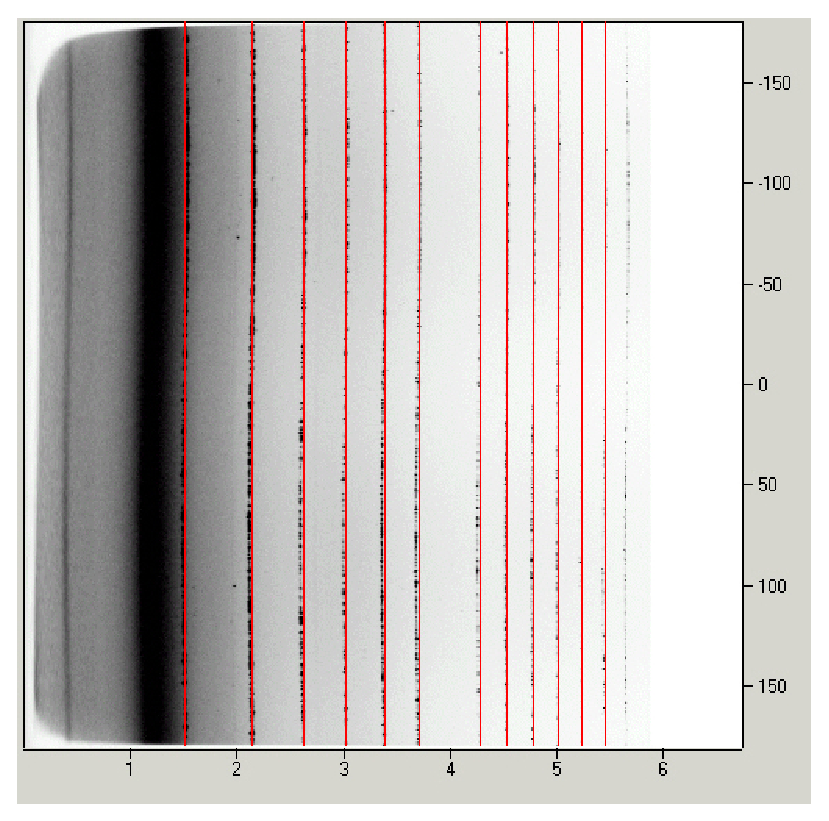
\includegraphics[scale=.75]
    {figures/bad_calibration_cake.eps}
    \caption{A cake with the calibration parameters
    found in the image header. These parameters
    are not particularly good and the diffraction peaks
    are not very straight.}
    \label{bad_calibration_cake}
\end{SCfigure}

\begin{SCfigure}[1][bthp]
    \centering
    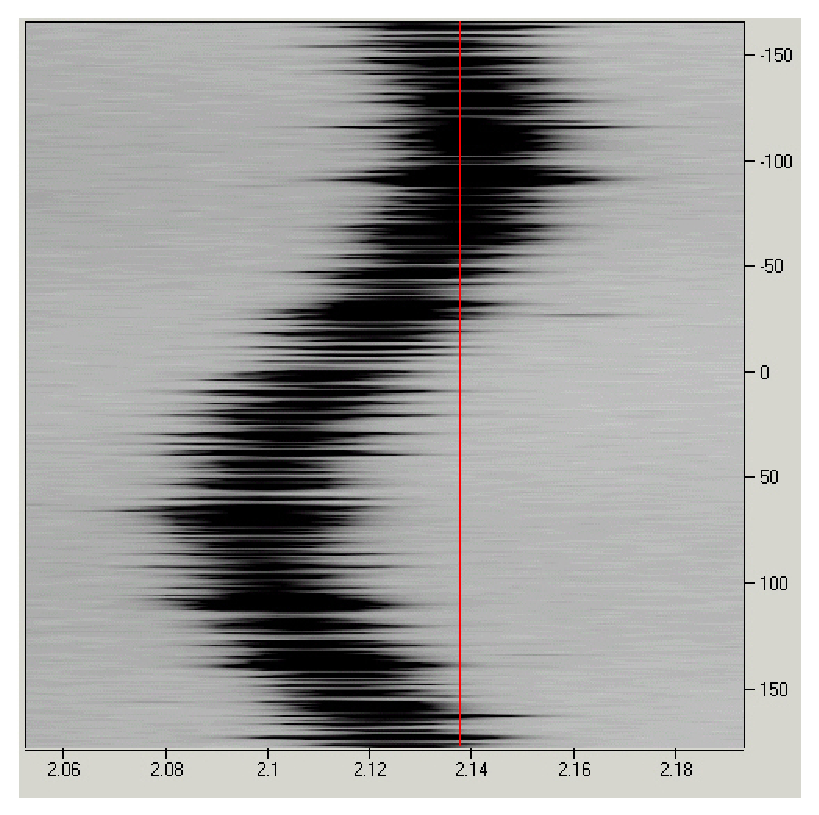
\includegraphics[scale=.75]
    {figures/bad_calibration_cake_zoom.eps}
    \caption{A zoom in of the cake shown in 
    figure~\ref{bad_calibration_cake}. The poor calibration 
    becomes much more obvious.}
    \label{bad_calibration_cake_zoom}
\end{SCfigure}

Calibration can be done with the \gui{Do Fit} button 
on the \gui{Calibration} tab. If the calibration is good, 
the constant $Q$ lines drawn on the diffraction image 
entirely overlap the real diffraction patter. 
A good calibration is shown in 
figure~\ref{good_calibration_diffraction_image}.
The peaks on the caked image also become much straighter.
Figure~\ref{good_calibration_cake} shows the caked data after calibration 
Figure~\ref{good_calibration_cake_zoom} shows that the peaks
look good even when zoomed in.
The calibration parameters can be saved to 
a file for later use using the \gui{Save to File} button on the 
\gui{Calibration} tab. 

\begin{SCfigure}[1][bthp]
    \centering
    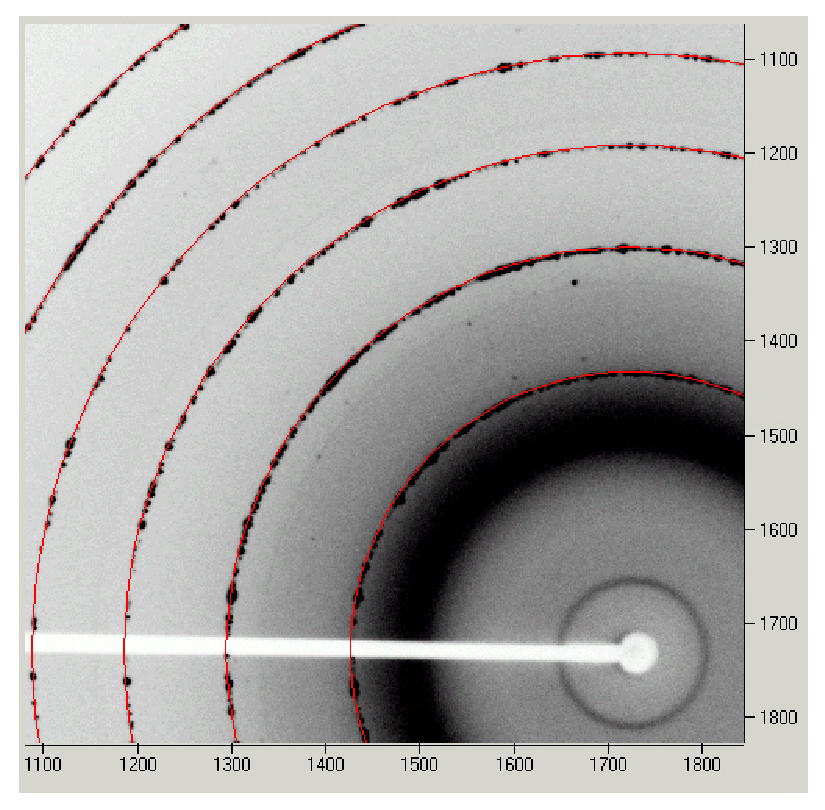
\includegraphics[scale=.75]
    {figures/good_calibration_diffraction_image.eps}
    \caption{The diffraction window after calibration. The
    constant $Q$ lines are on top of the diffraction 
    peaks.}
    \label{good_calibration_diffraction_image}
\end{SCfigure}

\begin{SCfigure}[1][bthp]
    \centering
    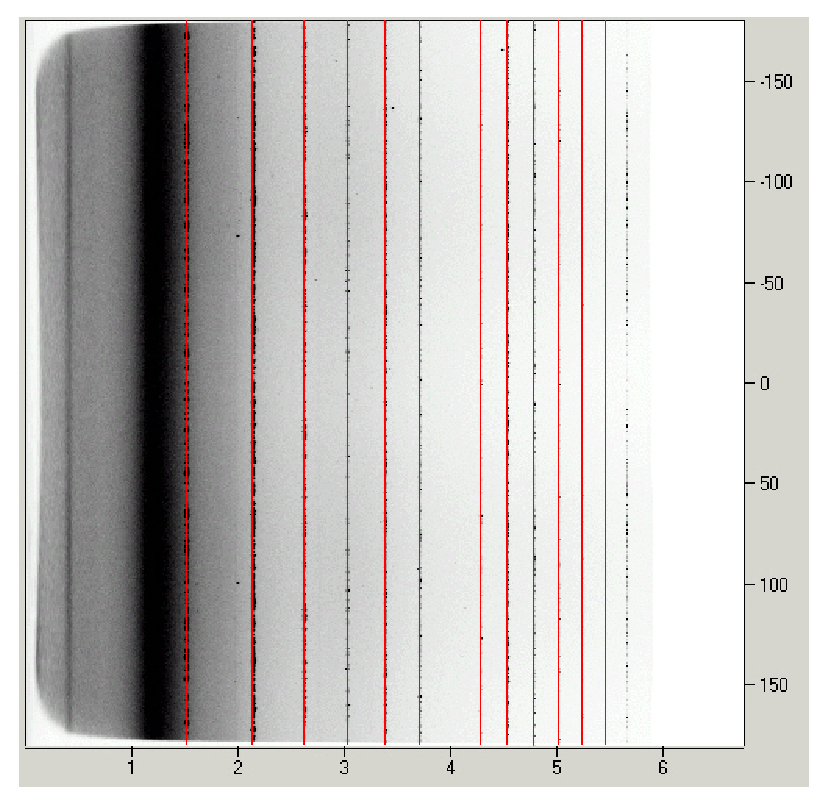
\includegraphics[scale=.75]
    {figures/good_calibration_cake.eps}
    \caption{The cake window after calibration.  The lines 
    are much straighter than before calibration.}
    \label{good_calibration_cake}
\end{SCfigure}

\begin{SCfigure}[1][bthp]
    \centering
    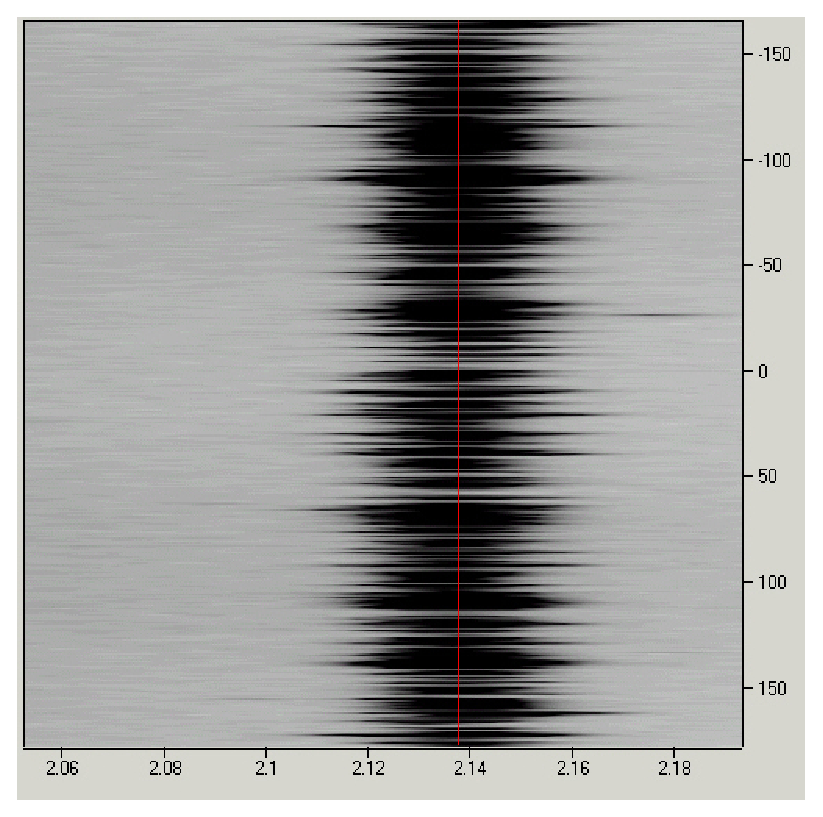
\includegraphics[scale=.75]
    {figures/good_calibration_cake_zoom.eps}
    \caption{The same zoom as in figure~\ref{good_calibration_cake}. 
    The line remains very straight.}
    \label{good_calibration_cake_zoom}
\end{SCfigure}

There is a beam stop in the image obstructing part of the data. 
It can be ignored with a polygon mask. Masking is done
on the \gui{Masking} tab. The masking tab is shown in 
figure~\ref{masking_tab_example}. Figure 
~\ref{masked_beam_stop} shows a rectangular mask covering
the beam stop.
The \gui{Save Mask} button can be used to save the mask
to a file. The mask can later be loaded into the program when
performing the rest of the analysis.

\begin{SCfigure}[1][bthp]
    \centering
    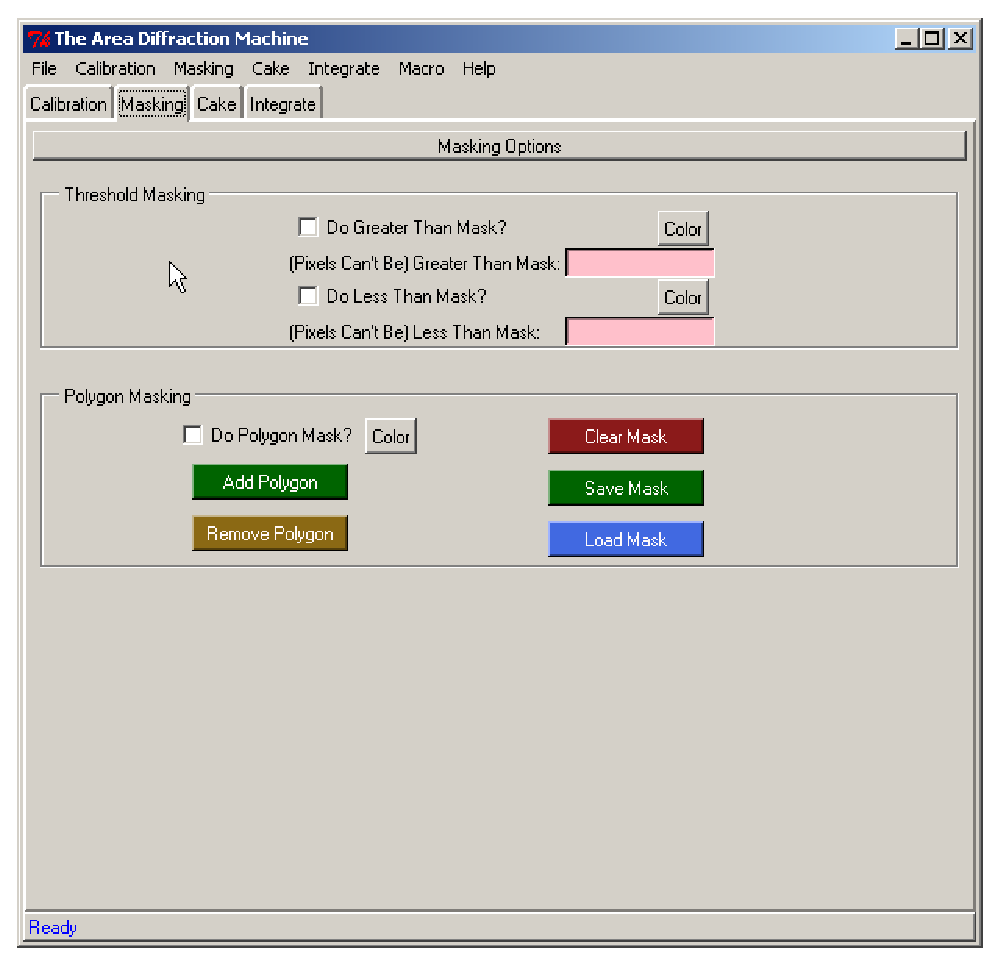
\includegraphics[scale=.75]
    {figures/masking_tab.eps}
    \caption{The pixel masking tab.}
    \label{masking_tab_example}
\end{SCfigure}

\begin{SCfigure}[1][bthp]
    \centering
    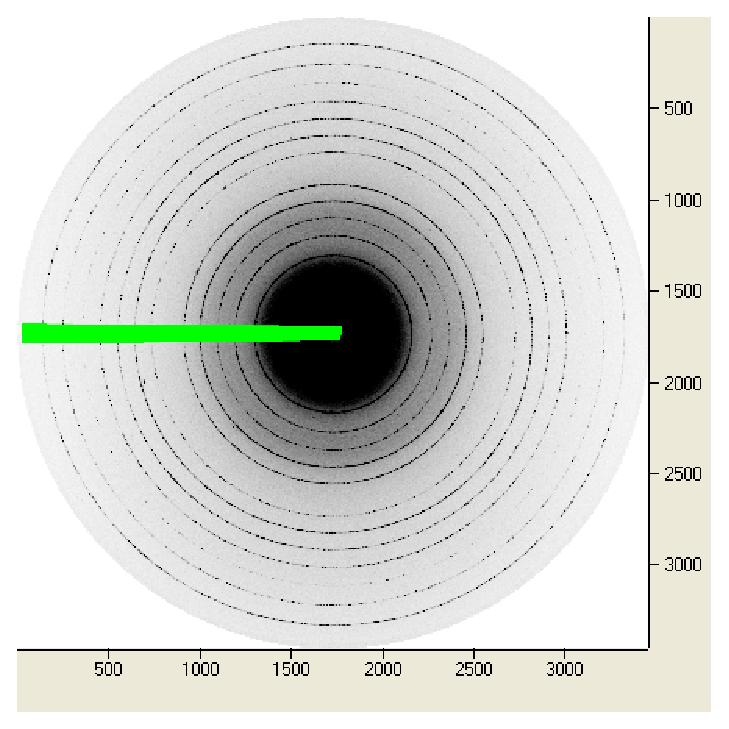
\includegraphics[scale=.75]
    {figures/masked_beam_stop.eps}
    \caption{A mask is drawn over the beam stop. It will ensure
    that the beam stop will not be used in subsequent analysis.}
    \label{masked_beam_stop}
\end{SCfigure}

After calibrating the detector and creating the beam stop mask, 
the rest of the data can be analyzed. This is done by 
performing an intensity integration on each of the other files.
To perform the integration, the diffraction file must first be loaded.
The calibration parameters determined earlier must be loaded and the
beam stop mask must be loaded. The \gui{Do Polygon Mask?} check box needs to
be selected to ensure that the polygon masks are used in the analysis.
Then, a $Q-I$ integration is done by pushing the \gui{AutoIntegrate} button 
on the left side of the \gui{Integration} tab
shown in figure~\ref{integration_tab_example}.
Intensity data for one of the iron samples is shown in 
figure~\ref{iron_intensity}.

\begin{SCfigure}[1][bthp]
    \centering
    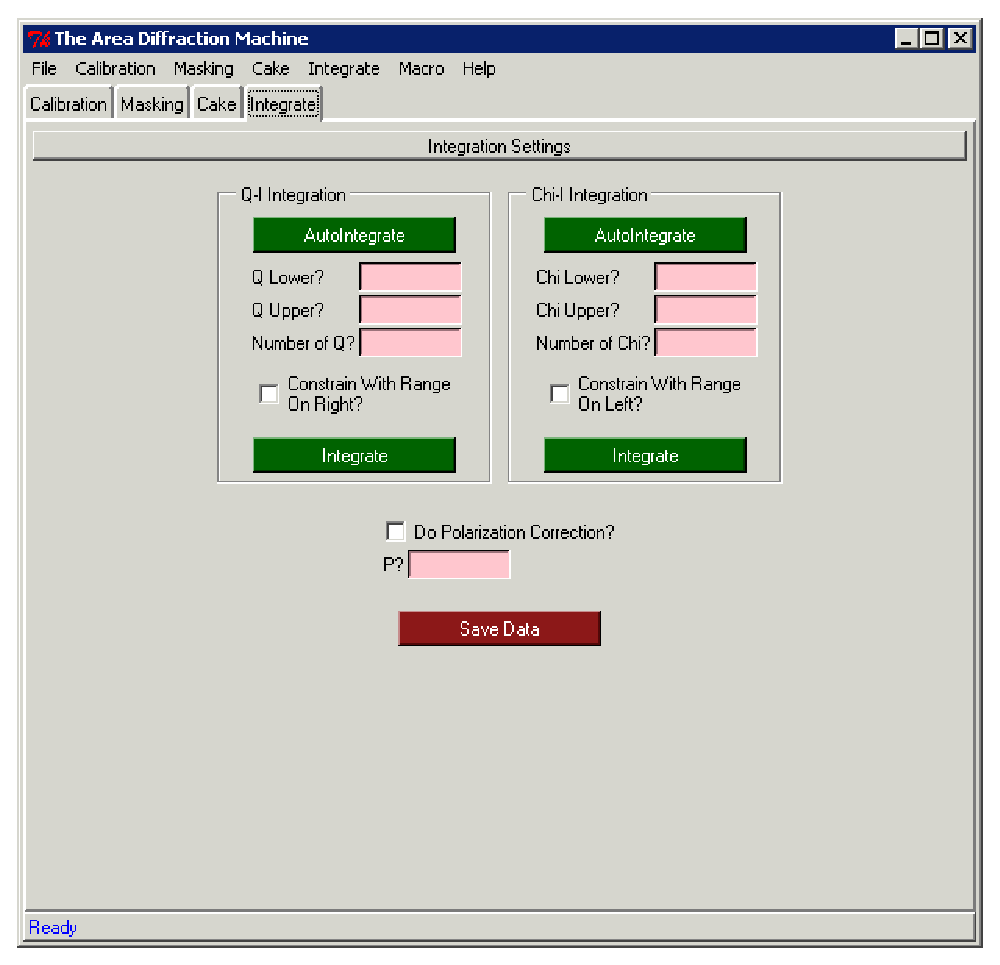
\includegraphics[scale=.75]
    {figures/integration_tab.eps}
    \caption{The integration tab.}
    \label{integration_tab_example}
\end{SCfigure}

\begin{SCfigure}[1][bthp]
    \centering
    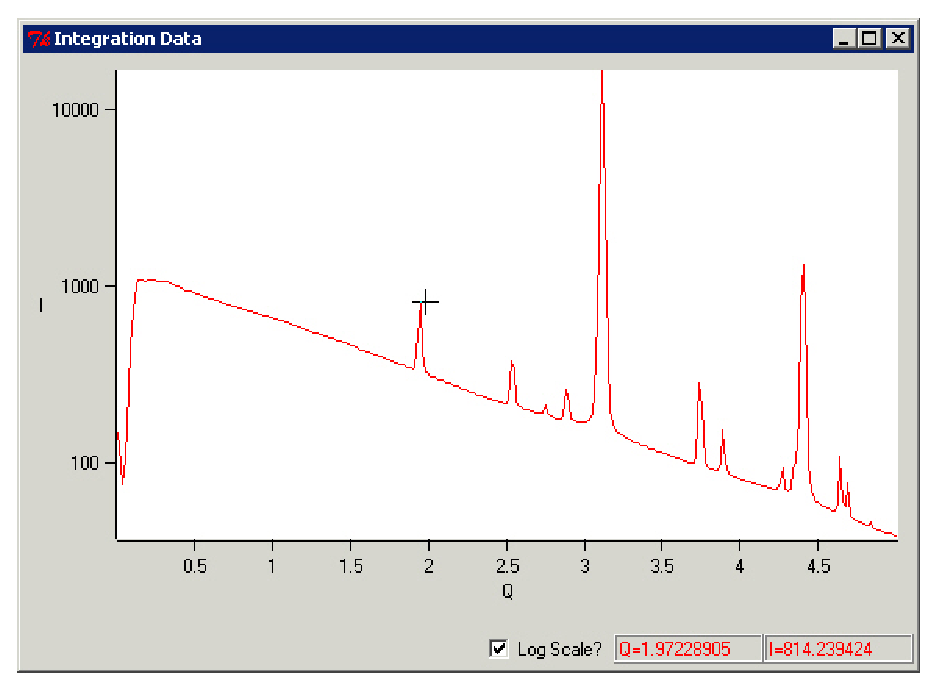
\includegraphics[scale=.75]
    {figures/iron_intensity.eps}
    \caption{The intensity integration window for 
    a particular iron sample.}
    \label{iron_intensity}
\end{SCfigure}

The intensity integrated data can be saved to a file
using the \gui{Save Data} button on the \gui{Integration} tab. 
The data is saved out as two column ASCII. This same 
process could be done to all the files that need to be 
analyzed. This would be very time consuming if there were a lot of files . 
If all of the data was in the folder \macroline{C:/Data/}, all the data 
it could all be analyzed using the macro
\begin{lstlisting}
Data File:
	C:/Data/
Load From File
    C:/Data/LaB6_cal.dat
Load Mask
    C:/Data/beam_stop_mask.dat
Do Polygon Mask?
    Select
AutoIntegrate Q-I
Save Integration Data
    PATHNAME/FILENAME_int.dat
\end{lstlisting}
The first command loads into the program all the
diffraction files in the folder \macroline{C:/Data/}
one at a time and runs the rest of the analysis on
each of them. The macro loads in the calibration parameters
and loads in the beam stop 
mask. It then does a $Q-I$ intensity integrated and 
saves the integration data to a file. 

After the macro is run, the intensity integrated data can be open 
in Excel. 
The diffraction patterns of different data files can be plotted on
the same graph to look for shifts in diffraction peaks. 
This data might look something like the graph 
in figure~\ref{excel_peak_shift}.

\begin{SCfigure}[1][bthp]
    \centering
    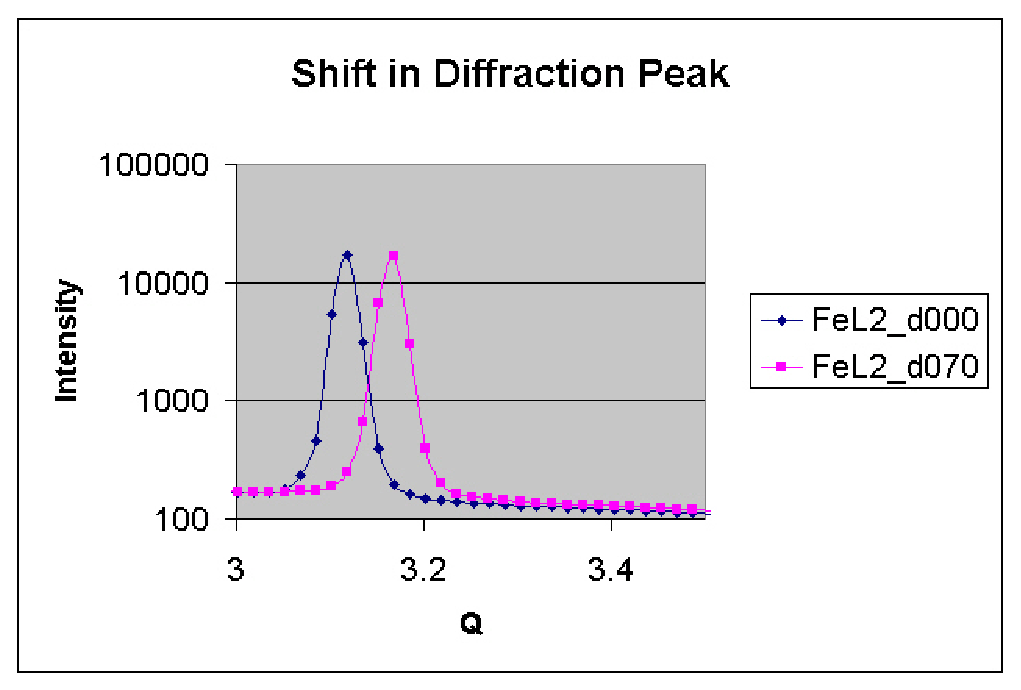
\includegraphics[scale=.5]
    {figures/excel_peak_shift.eps}
    \caption{What the shift in diffraction peaks might
    look like when two diffraction patterns are plotted
    on top of one another in Excel.}
    \label{excel_peak_shift}
\end{SCfigure}
